\documentclass[12pt,a4paper]{article}
\usepackage{pgf}
% \usepackage[condensed,math]{kurier}
% \usepackage[T1]{fontenc}
\usepackage{svg}
\usepackage{tikz}
\usepackage{stanli}
\usepackage{afterpage}
\usepackage{multirow}
\usepackage{subfig}
\usepackage{pgfpages}
\usepackage{float}
\usepackage{listings}
\usepackage{rotating}
\usepackage{bookmark}

\usepackage{hyperref}

\usepackage{xcolor}
\usepackage{svg}
\definecolor{codegreen}{rgb}{0,0.6,0}
\definecolor{codegray}{rgb}{0.5,0.5,0.5}
\definecolor{codepurple}{rgb}{0.58,0,0.82}
\definecolor{backcolour}{rgb}{0.95,0.95,0.92}

\lstdefinestyle{mystyle}{
    backgroundcolor=\color{backcolour},   
    commentstyle=\color{codegreen},
    keywordstyle=\color{magenta},
    numberstyle=\tiny\color{codegray},
    stringstyle=\color{codepurple},
    basicstyle=\ttfamily\footnotesize,
    breakatwhitespace=false,         
    breaklines=true,                 
    captionpos=b,                    
    keepspaces=true,                 
    numbers=left,                    
    numbersep=5pt,                  
    showspaces=false,                
    showstringspaces=false,
    showtabs=false,                  
    tabsize=2
}

\lstset{style=mystyle}

%\usepackage{times}


\pgfpagesdeclarelayout{boxed}
{
	\edef\pgfpageoptionborder{0pt}
}
{
	\pgfpagesphysicalpageoptions
	{%
		logical pages=1,%
	}
	\pgfpageslogicalpageoptions{1}
	{
		border code=\pgfsetlinewidth{2pt}\pgfstroke,%
		border shrink=\pgfpageoptionborder,%
		resized width=.9\pgfphysicalwidth,%
		resized height=.9\pgfphysicalheight,%
		center=\pgfpoint{.5\pgfphysicalwidth}{.5\pgfphysicalheight}%
	}%
}

\pgfpagesuselayout{boxed}


% Language setting
% Replace `english' with e.g. `spanish' to change the document language
\usepackage[english]{babel}
\usepackage{csvsimple}
% Set page size and margins
% Replace `letterpaper' with `a4paper' for UK/EU standard size
\usepackage[a4paper,top=2cm,bottom=1.5cm,left=1.5cm,right=1.5cm]{geometry}

% Useful packages
\usepackage{amsmath}
\usepackage{graphicx}

\title{}
\author{}
\date{}


\begin{document}

\newcommand{\subf}[2]{%
    {\small\begin{tabular}[t]{@{}c@{}}
                #1 \\#2
            \end{tabular}}%
}

\begin{titlepage}
    \begin{center}
        \vspace*{3cm}

        \Huge
        \textbf{Massive Parallel Cracker}

        \vspace{0.3cm}
        \Huge
        MD5

        \vspace{0.8cm}
        \large

        %INSTRUCTED BY: MRS. A.A.S.KAUSHLYA


        \vspace{0.5cm}
        \LARGE


        \vspace{1.5cm}

        \textbf{}
        %\includegraphics[width=0.8\textwidth]{./Images/model.png}

        \vfill



        \vspace{0.8cm}



        \Large




    \end{center}
    \Large
    \begin{tabbing}
        \hspace*{1em}\= \hspace*{8em} \= \kill % set the tabbings
        \> Name:\>  \textbf{Matteo Ielacqua} \\
        \> ID:\>  \textbf{839241} \\
    \end{tabbing}

\end{titlepage}


\section{Introduction}
MPC (Massive Parallel hash Cracker) is an MPI, MultiThreaded and GPU enabled software that let the user to try different password combination on a single hash using all the power of the distributed computing. The program is developed as an extensible example of how implement a distributed hash calculator.

\subsection{Hashing algorithm}
An hashing algorithm is a function that takes as input some bytes, usually divided in blocks of fixed length, and returns an array of bytes of fixed length. Examples of those functions are MD4/5 (a.k.a Message Digests algorithms), SHA-1/2/256/512. Tipically those kinds of functions serve the purpose to store password as encrypted hashes in a database, so that the authentication is done against the hash and not against the password in clear form. 

\subsection{MD5}
MD5 is a fast, efficient but not secure hashing algorithm. All hashing algorithm are designed with the intent to provide a specific and stable \(i.e of constant length\) output for all kind of inputs, but since they lack a mathematical proof of their behaviour we are satisfied to assume they work until the contrary is proven. That is the case for MD5, which a collision was found in 2004, and since then it is not considered a secure hashing algorithm, hovewer due to its simplicity it is still used in some applications like message digesting in non safety critical protocols.

\section{The application}
Develop an application to parallelize in hashing algorithm is the target of many hackaton, many applications surrounding the SHA-1 and SHA-256 algorithms were written, usually combining both GPU and CPU load. In this istance my objective was quite simple: write an application that can calculate a password stored as MD5 using a bruteforce attack.

\subsection{Tools and languages used}
The project is divided in 2 parts: the libraries and the core. Under the libraries there are 2 implementation of the MD5 hashing algorithm, one for the cpu with also a string generator written both in C,  and the other for the gpu written in CUDA with a compatible string generator. The core program is written in C++ using MPI, Pthread and OpenMP.


\subsection{Brief description of the libraries}
The libraries hold the implementation of the MD5 algorithm and the string generator for the bruteforce mode.

\subsubsection{CPU Version}
In the CPU version it is only necessary to supply an arbitrary string to the function 
\begin{lstlisting}
    void md5String(char *input, uint8_t *result);
\end{lstlisting}

The computed result of 16 bytes will be returned. This implementation of the MD5 algorithm works as intended by the literature, so a string of characters is shuffled (using different bitwise operations) with a magic table that provide the constant used in the hashing algorithm. Each step of the algorithm is performed on 512 bit of input, that are padded when the remained characters are less than this measure.

\begin{lstlisting}
    void md5Step(uint32_t *buffer, uint32_t *input){
        uint32_t AA = buffer[0];
        uint32_t BB = buffer[1];
        uint32_t CC = buffer[2];
        uint32_t DD = buffer[3];
        uint32_t E;
        unsigned int j;
        for(unsigned int i = 0; i < 64; ++i){
            switch(i / 16){
                case 0:
                    E = F(BB, CC, DD);
                    j = i;
                    break;
                case 1:
                    E = G(BB, CC, DD);
                    j = ((i * 5) + 1) % 16;
                    break;
                case 2:
                    E = H(BB, CC, DD);
                    j = ((i * 3) + 5) % 16;
                    break;
                default:
                    E = I(BB, CC, DD);
                    j = (i * 7) % 16;
                    break;
            }
            uint32_t temp = DD;
            DD = CC;
            CC = BB;
            BB = BB + rotateLeft(AA + E + K[i] + input[j], S[i]);
            AA = temp;
        }
        buffer[0] += AA;
        buffer[1] += BB;
        buffer[2] += CC;
        buffer[3] += DD;
    }
\end{lstlisting}

The string generator instead is a container of all possible permutation of a string of visible characters in utf8 so in the range $ [!(33) , tilde (126)]$. 

\begin{lstlisting}
    struct SequenceGeneratorCtx new_seq_generator(uint8_t base_len);
    void seq_gen_next_sequence(struct SequenceGeneratorCtx* ctx);
    void seq_gen_skip_to(struct SequenceGeneratorCtx* ctx,size_t address);
\end{lstlisting}

The generator works using 2 algorithms, one that is a combinatorial search so that the user can target a specific string by expressing it as an offset from the string ``!'' 

\begin{lstlisting}
    void seq_gen_skip_to(struct SequenceGeneratorCtx* ctx,uint64_t address)
{
    int div = maxCharint - minCharInt;
    int q = address;
    int r = 0;
    int it = 0;
    while (q > 0)
    {
        r = q % div;
        q /= div;
        if (it == ctx->current_len)
        {
            shift_buffer(ctx->buffer, ctx->current_len, 1); 
            ctx->current_len++;
            ctx->buffer[0] = minCharInt;
        }
        ctx->buffer[ctx->current_len - it - 1] = (char)(r + minCharInt);
        it++;
    }
}

\end{lstlisting}


\subsubsection{GPU Version}
The GPU version of the MD5 algorithm is a porting of the CPU one with some modifications to minimize the memory transfers needed.

\begin{lstlisting}
    struct Md5TransformResult{
    char* data;
    size_t size;
}; 
struct Md5BruterResult{
    char data[33];
    bool found;
};
struct Md5TransformResult md5_gpu(char* data, uint8_t * sizes, size_t array_size, int maxthreads);
struct Md5BruterResult md5_bruter(size_t start_address, size_t end_address, const char* target_md5, int maxthreads);
\end{lstlisting}

The first function calculate a vector of digests from a vector of strings, without doing any comparison. The second function instead take an interval of addresses for the string generator and return the string that generate the hash if in the given span the target md5 is found, this function require a really tiny memory transfer compared to the first one , because the comparison is done directly in the GPU and the user need only to allocate and copy 8+8+32 byte in the GPU memory : start, end and target\_md5.

\section{Brief description of the core}
The core implements all the communication procedures between the MPI nodes , the loader for the configuration file and the computation functions that wrap around the MD5 algorithms. The core also organize how the nodes are connected between each other.
\\
\begin{figure}[H]
    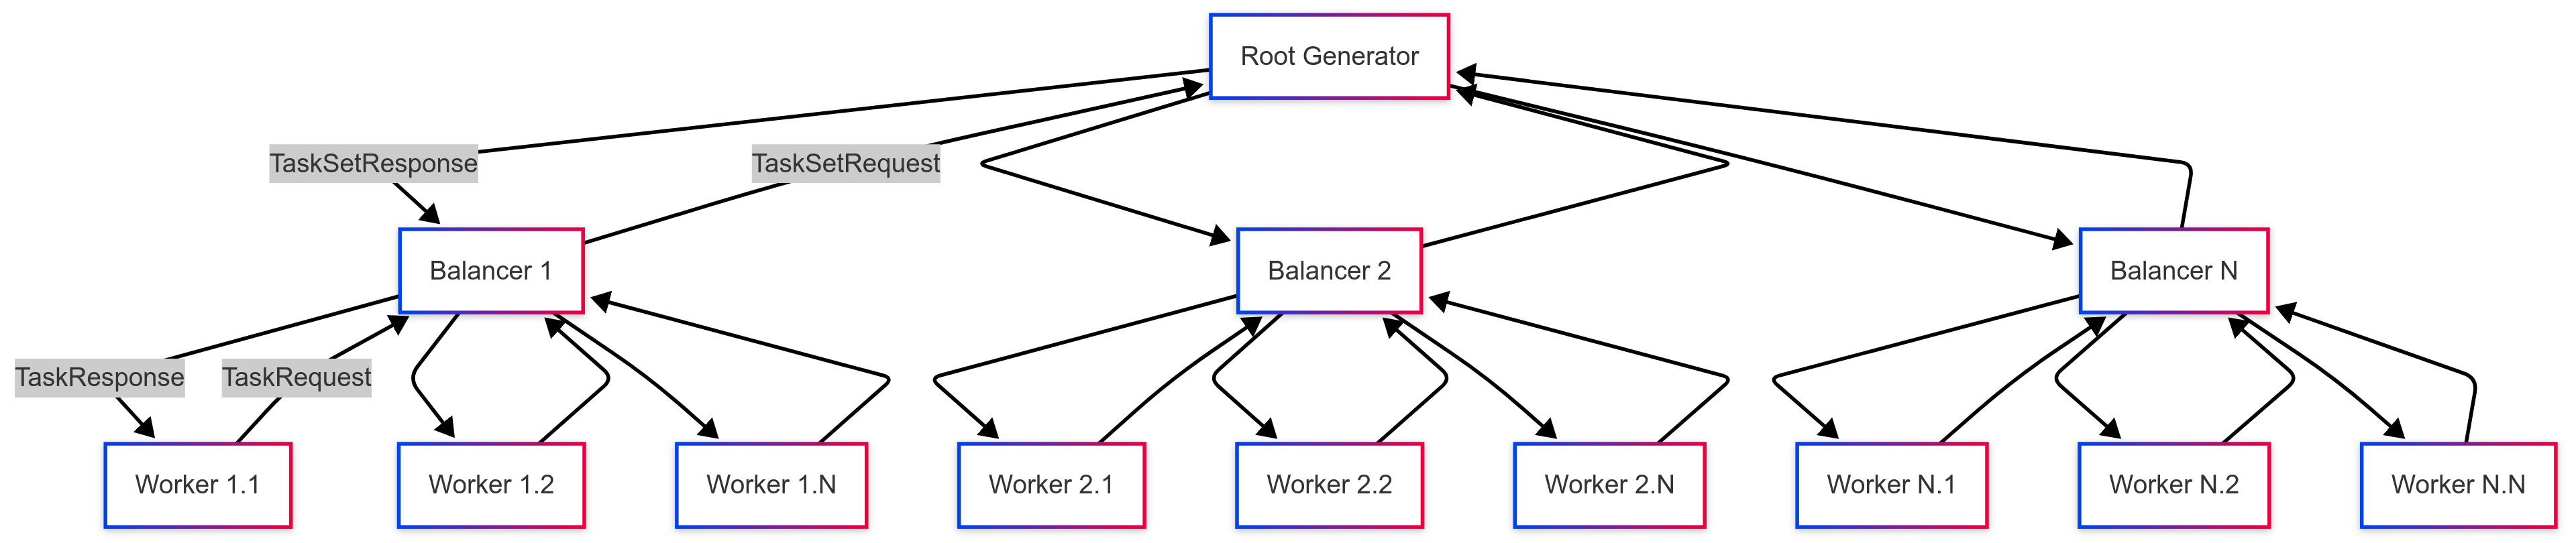
\includegraphics[width=0.9\textwidth]{images/diagram_with_balancers.png}
    \caption{Diagram of nodes interactions}
\end{figure}

Using the cluster degree is possible to specify how many balancers there are in the network , if 0 then all the workers are connected to the master. 

\subsection{Master}

The master generate the tasks as a pair of addresses both 64 bit longs to feed the string generators, those are generated only when a balancer or a worker requests one or more task by sending a message to the master, if balancers are present in the network then only those nodes will requests a task to the master.

\subsection{Balancer}
The balancers are an optional kind of node, their presence can be specified using the cluster degree parameter inside the configuration file. When the network is built the master assign a number of workers less or equal to $\frac{size-1}{balancers}$ to each balancer

\subsection{Workers}
The workers are the computational part of the processes. When the network is build at each worker is assigned a balancer, or in their absence, the master, during this base a GPU is chosen between the available ones based on the rank of the process. When a worker start it's routine it immediately ask for a task to a master or balancer, workers always require 1 task at a time. When a task is received , the computation start immediately on the assigned GPU if enabled, else the computation is performed using the CPU with the task divided in chunk specified by the user through the cpu_threads and chunk parameters.


\section{Theoretical expectations}



\end{document}

